\documentclass[12pt]{article}

\usepackage{graphicx,amsmath,textcomp,caption,subcaption,cite}
\usepackage[round]{natbib}
\usepackage[margin=2cm]{geometry}
%\usepackage[subtle]{savetrees}
\linespread{1.1}
\bibliographystyle{plainnat}
\title{
ENGN1218 Introduction to Electronics\\
Full-wave Rectifier Analysis\\
}
\author{
\and Paul Apelt, u5568225
\and Thomas Hale, u5567957
\and School of Engineering, ANU 
}
\begin{document}
\maketitle
\begin{abstract}
A diode-bridge full wave power rectifier circuit was designed and constructed. The aim was to achieve a 12V DC output with 10\% tolerance. A theoretical analysis of two types of diode-bridge full-wave rectifiers---with and without a capacitor---was conducted, and results confirmed using a computer simulation. The construction process was documented, and all output parameters measured. The aim was successfully achieved, with all output parameters matching the predicted values within an acceptable error bound.
\end{abstract}
\section{Introduction}
\label{sec:int}
\section{Theoretical Analysis}
\label{sec:the}
Two versions of a full-wave rectifier circuit were analysed, with and without a smoothing capacitor, schematics shown in Figures \ref{fig:cap} and \ref {fig:nocap} respectively.
\begin{figure}[h!]
\centering
\begin{subfigure}[b]{0.45\textwidth}
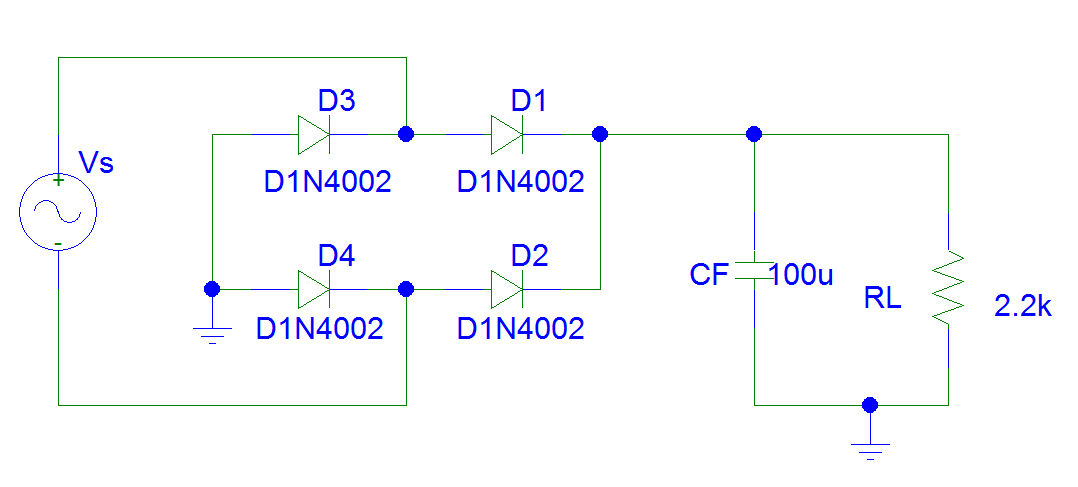
\includegraphics[width=\textwidth]{rekt_cap}
\caption{Full-wave rectifier with a capacitor filter.}
\label{fig:cap}
\end{subfigure}
\qquad
\begin{subfigure}[b]{0.45\textwidth}
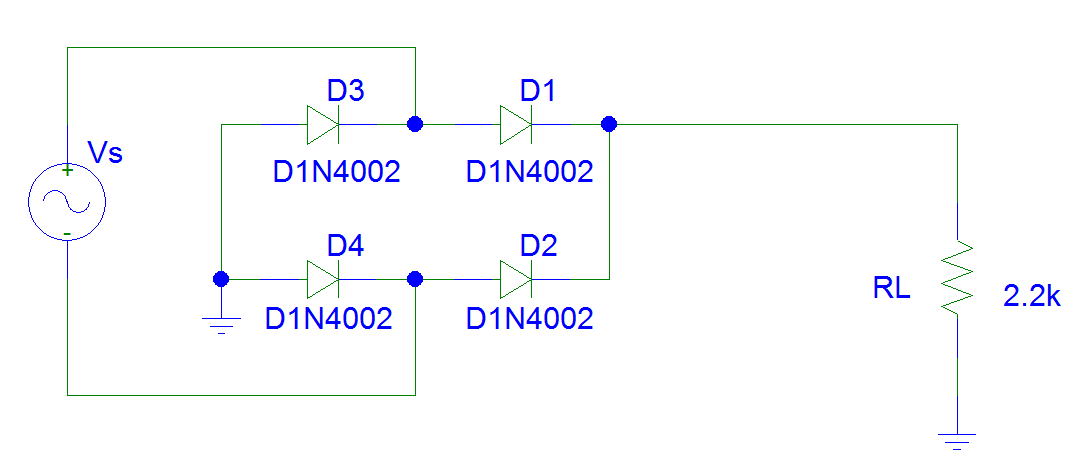
\includegraphics[width=\textwidth]{rekt_nocap}
\caption{Full-wave rectifier without a capacitor filter.}
\label{fig:nocap}
\end{subfigure}
\caption{Schematics.}
\label{fig:sch}
\end{figure}

To predict the output of the rectifier circuit, formulas from the textbook were used \citep{textbook}. The value for the input voltage $V_{in}$\footnote{Unless explicitly stated otherwise, all AC voltage values are peak-to-peak.} was taken to be equal to the actual output of the transformer used during testing (see Section~\ref{sec:imp}). The output voltage of a rectifier without a capacitor filter was calculated in Equation~\ref{eq:nocap}, and the voltage ripple of the output of the rectifier with a smoothing capacitor---in Equation~\ref{eq:cap}.
\begin{align}
\begin{split}
V_{out}&=V_{in}-2\times0.7\\
&=18.8-1.4\\
&=17.4\mathrm{V}
\label{eq:nocap}
\end{split}
\end{align}

Note that in the above case, in the absence of the smoothing capacitor, $V_r=V_{out}$. The addition of a capacitor has no effect on the output peak voltage, but decreases ripple.
\begin{align}
\begin{split}
V_{r}&=\frac{V_{out}}{2f R_L C}\\
&=\frac{17.4}{2\times50\times2.2\times10^3\times10^{-4}}\\
&\approx0.79\mathrm{V}
\label{eq:cap}
\end{split}
\end{align}

\section{Simulation}
\label{sec:sim}
\section{Implementation}
\label{sec:imp}
\section{Discussion}
\label{sec:dis}
\section{Conclusion}
\label{sec:con}
\bibliography{electronics.bib}
\end{document}
